\chapter{计算智能}

\begin{question}
计算智能的含义是什么?它涉及哪些研究分支?
\end{question}
\begin{solution}
贝兹德克认为计算智能取决于制造者提供的数值数据,而不依赖于知识;另一个方面,人工智能则应用知识精品。计算智能是一种智力方式的低层认知,它与人工智能的区别只是认知层次从中层下降至底层而已。中层系统含有知识(精品),底层系统则没有。它与人工智能的主要区别在于它不含知识精品。\par
计算智能主要的研究领域为神经计算,模糊计算,进化计算,人工生命。 
\end{solution}

\begin{question}
试述计算智能(CI)、人工智能(AI)和生物智能(BI)的关系。
\end{question}
\begin{solution}
计算智能是智力的低层认知,主要取决于数值数据而不依赖于知识。人工智能是在计算智能的基础上引入知识而产生的智力中层认知。生物智能,尤其是人类智能,则是最高层的智能。\par
A- Artificial,表示人工的(非生物的);\par
B- Biological,表示物理的+化学的+(?)=生物的;\par
C- Computational,表示数学+计算机。\par
CI智能是最低的,它没有知识,就是数据计算。从复杂性来看,BI$>$AI$>$CI;从所属关系来看,CI$\subset$AI$\subset$BI;AI是CI到BI的过渡,因为AI中除计算算法之外,还包括符号表示及数值信息处理。\par
计算智能是一种智力方式的低层认知,它与人工智能的区别只是认知层次从中层下降至低层而已。中层系统含有知识,低层系统则没有。
\end{solution}

\begin{question}
人工神经网络为什么具有诱人的发展前景和潜在的广泛应用领域?
\end{question}
\begin{solution}
人工神经网络具有如下至关重要的特性:
	\begin{enumerate}
		\item 并行分布处理 \\
神经网络具有高度的并行结构和并行实现能力,因为具有较好的耐故障能力和较快的总体处理能力。这一特性特别适于实时和动态处理。
		\item 非线性映射 \\
神经网络具有固有的非线性特性,这源于其近似任意非线性映射(变换)能力。这一特性给处理非线性问题带来新的希望。
		\item 通过训练进行学习 \\
神经网络是通过所研究系统过去的数据记录进行训练的。一个经过适当训练的神经网络具有归纳全部数据的能力。因此,神经系统能够解决那些由数学模型或描述规则难以处理的问题。
		\item 适应与集成 \\
神经网络能够适应在线运行,并能同时进行定量和定性操作。神经网络的强适应和信息融合能力使得它可以同时输入大量不同的控制信号,解决输入信息间的互补和冗余问题,实现信息集成和融合处理。这些特性特别适于复杂、大规模和多变量系统。
		\item 硬件实现 \\
神经网络不仅能够通过软件而且可以借助硬件实现并行处理。近年来,一些超大规模集成电路实现硬件已经问世,而且可以从市场上购买到。这使得神经网络成为具有快速和大规模处理能力的网络。
	\end{enumerate} \par
	显然,神经网络由于其学习和适应、自组织、函数逼近和大规模并行处理等能力,因而具有用于智能系统的潜力。\par
	神经网络在模式识别、信号处理、系统辨识和优化等方面的应用,已有广泛研究。在控制领域,已经做出许多努力,把神经网络用于控制系统,处理控制系统的非线性和不确定性以及逼近系统的辨识函数等。
\end{solution}

\begin{question}
简述生物神经元及人工神经网络的结构和主要学习算法。
\end{question}
\begin{solution}
生物神经元的结构:\par
大多数神经元由一个细胞体(cell body或soma)和突触(process)两部分组成。突触分两类, 即轴突(axon)和树突(dendrite),轴突是个突出部分,长度可达1m,把本神经元的输出发送至其它相连接的神经元。树突也是突出部分,但一般较短,且分枝很多,与其它神经元的轴突相连,以接收来自其它神经元的生物信号。\par
轴突的末端与树突进行信号传递的界面称为突触(synapse),通过突触向其它神经元发送信息。对某些突触的刺激促使神经元触发(fire)。只有神经元所有输入的总效应达到阈值电平,它才能开始工作。此时,神经元就产生一个全强度的输出窄脉冲,从细胞体经轴突进入轴突分枝。这时的神经元就称为被触发。突触把经过一个神经元轴突的脉冲转化为下一个神经元的兴奋或抑制。学习就发生在突触附近。\par
每个人脑大约含有1011-1012个神经元,每一神经元又约有103-104个突触。神经元通过突触形成的网络,传递神经元间的兴奋与抑制。大脑的全部神经元构成极其复杂的拓扑网络群体,用于实现记忆与思维。\par
人工神经网络的结构:\par
人工神经网络由神经元模型构成。每个神经元具有单一输出,并且能够与其它神经元连接,存在许多输出连接方法,每种连接方法对应于一个连接权系数。人工神经网络的结构分为2类:
	\begin{enumerate}
	\item 递归(反馈)网络 \\
有些神经元的输出被反馈至同层或前层神经元。信号能够从正向和反向流通。Hopfield网络,Elmman网络和Jordan网络是代表。 
	\item 前馈网络 \\
具有递阶分层结构,由一些同层神经元间不存在互连的层级组成。从输入层至输出层的信号通过单向连接流通,神经元从一层连接至下一层,不存在同层神经元之间的连接。多层感知器(MLP),学习矢量量化网络(LVQ),小脑模型连接控制网络(CMAC)和数据处理方法网络(GMDH)是代表。
	\end{enumerate} \par
人工神经网络的主要学习算法:
	\begin{enumerate}
	\item 指导式(有师)学习 \\
根据期望和实际的网络输出之间的差来调整神经元连接的强度或权。包括Delta规则,广义Delta规则,反向传播算法及LVQ算法。 
	\item 非指导(无导师)学习 \\
训练过程中,神经网络能自动地适应连接权,以便按相似特征把输入模式分组聚集。包括Kohonen算法,Carpenter-Grossberg自适应谐振理论(ART)。 
	\item 强化学习 \\
是有师学习的一种特例。它不需要老师给出目标输出,而是由一个“评论员”来评介与给定输入相对应的神经网络输出的优度。例如遗传算法(GA)。  
	\end{enumerate}	 
\end{solution}

\begin{question}
考虑一个具有阶梯形阈值函数的神经网络,假设
	\begin{enumerate}
		\item 用一常数乘所有的权值和阈值;
		\item 用一常数加所有的权值和阈值。
	\end{enumerate}
试说明网络性能是否会变化?
\end{question}
\begin{solution}
	\begin{enumerate}
		\item 不会。
		\item 会。
	\end{enumerate}
\end{solution}

\begin{question}
构作一个神经网络,用于计算含有两个输入的XOR函数。指定所用神经网络单元的种类。
\end{question}
\begin{solution}
已知用单层感知机是无法解决XOR问题的,需要增加隐单元。隐单元的数量可以有多种选择。这里给出含有两个隐单元(只有一层隐单元)的前馈神经网络。\par 
	\begin{figure}[h]
		\centering
		\def\layersep{2.5cm}

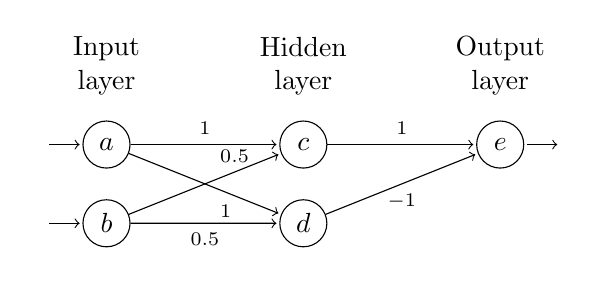
\begin{tikzpicture}[shorten >=1pt,->,draw=black, node distance=\layersep,
	every edge/.append style={nodes={font=\scriptsize}}]
    \tikzstyle{every pin edge}=[<-,shorten <=1pt]
    \tikzstyle{neuron}=[circle,draw=black,minimum size=17pt,inner sep=0pt]
    \tikzstyle{input neuron}=[neuron];
    \tikzstyle{output neuron}=[neuron];
    \tikzstyle{hidden neuron}=[neuron];
    \tikzstyle{annot} = [text width=4em, text centered]

    % Draw the input layer nodes
    %\foreach \name / \y in {1,...,2}
    % This is the same as writing \foreach \name / \y in {1/1,2/2,3/3,4/4}
        \node[input neuron, pin=left:] (I-1) at (0,-1) {$a$};
        \node[input neuron, pin=left:] (I-2) at (0,-2) {$b$};

    % Draw the hidden layer nodes
    %\foreach \name / \y in {1,...,2}
        \node[hidden neuron] (H-1) at (\layersep,-1 cm) {$c$};
        \node[hidden neuron] (H-2) at (\layersep,-2 cm) {$d$};

    % Draw the output layer node
    \path[yshift=0.5cm]
    		node[output neuron,pin={[pin edge={->}]right:}, right of=H-1] (O) {$e$};

    % Connect every node in the input layer with every node in the
    % hidden layer.    
    \path (I-1) edge node[above]{$1$} (H-1);
    \path (I-1) edge node[above=10pt,right=2pt]{$0.5$} (H-2);
    \path (I-2) edge node[below=10pt,right=2pt]{$1$} (H-1);
    \path (I-2) edge node[below]{$0.5$} (H-2);

    % Connect every node in the hidden layer with the output layer
    \path (H-1) edge node[above]{$1$} (O);
    \path (H-2) edge node[below]{$-1$} (O);

    % Annotate the layers
    \node[annot,above of=H-1, node distance=1cm] (hl) {Hidden layer};
    \node[annot,left of=hl] {Input layer};
    \node[annot,right of=hl] {Output layer};
\end{tikzpicture}
		\caption{XOR问题的神经网络} \label{Fig:NN-XOR}
	\end{figure}
支持XOR问题的神经网络可以如图\ref{Fig:NN-XOR}所示。在这个神经网络中,共有5个处理单元,其中,$a$和$b$是输入单元,$c$和$d$是隐单元,它们位于网络的同一层上,$e$是输出单元。各单元的作用函数$O_i = f(a_i)$为阈值型。
\[O_i = \begin{cases}
	1, \quad a_i \geq 1 \\
	0, \quad a_i < 1
\end{cases} \]
\end{solution}

\begin{question}
假定有个具有线性激励函数的神经网络,即对于每个神经元,其输出等于常数$c$乘以各输入加权和。
	\begin{enumerate}
		\item 设该网络有个隐含层。对于给定的权$W$,写出输出层单元的输出值,此值以权$W$和输入层$I$为函数,而对隐含层的输出没有任何明显的叙述。试证明:存在一个不含隐含单位的网络能够计算上述同样的函数。
		\item 对于具有任何隐含层数的网络,重复进行上述计算。从中给出线性激励函数的结论。
	\end{enumerate}
\end{question}
\begin{solution}
为简单起见,这里假设在每个单元激励函数为相同的线性函数:$g(x)=cx+d$(如果对每个单元允许不同的$c_i$和$d_i$是一样的)。
	\begin{enumerate}
	\item 隐含层的输出为
	\[ H_j = g \left( \sum\limits_k W_{kj} I_k \right) = c \sum\limits_k W_{kj} I_k + d \, ,\]
	最终的输出为
	\[ O_i = g \left( \sum\limits_j W_{ji} H_j \right) = c \left( \sum\limits_j W_{ji} \left( c \sum\limits_k W{kj} I_k + d \right) \right) + d \, ,\]
	对于该输出,可以看出实际上可以化为输入的线性关系:
	\[ O_i = c^2 \sum\limits_k I_k \sum\limits_j W_{kj} W_{ji} + d \left( 1 + c \sum\limits_j W_{ji} \right) 、, . \]
	这样,就可以只使用一层感知机计算和两层网络相同的函数,其权重和激励函数分别为:
	\[ W_{ki} = \sum\limits_j W_{kj} W_{ji} \, ,\]
	\[ g(x) = c^2 + d \left( 1+c \sum\limits_j W_{ji} \right) \, .\]
	\item 上述归约可以将n层网络归约为$n-1$网络。归纳得出,n层网络可以归约为单层网络。这样,线性激励函数使得神经网络只能表示线性的函数。
	\end{enumerate}
\end{solution}

\begin{question}
什么是模糊性?它的对立含义是什么?试各举出两个例子加以说明。
\end{question}
\begin{solution}
模糊性指的是事物特性未被真实展现。它的对立含义是客观真实性。比如人到中年具有模糊性,人们对``中年''的理解并不是精确的一个岁数。58岁是一个精确的岁数。
\end{solution}

\begin{question}
什么是模糊集合和隶属函数或隶属度?
\end{question}
\begin{solution}
模糊集合是用来表达模糊性概念的集合,又称模糊集、模糊子集。设$U$为某些对象的集合,称为论域,可以是连续的或离散的;$u$表示$U$的元素,记作$U={u}$。论域$U$到$[0,1]$区间的任一映射$\mu_F$,即$\mu_F \colon U\to [0,1]$,都确定U的一个模糊子集$F$;$\mu_F$称为$F$的隶属函数或隶属度。
\end{solution}

\begin{question}
模糊集合有哪些运算?满足哪些规律?
\end{question}
\begin{solution}
模糊集合的交、并、补。设$A$、$B$是论域$U$上的两个模糊集,分别称$A \cup B$、$A \cap B$为$A$与$B$的并集、交集,称$\overline{A}$为$A$的补集,它们的隶属函数分别为:
	\begin{align*}
		\mu_{A \cup B}(u) &= \max \left\{ \mu_A(u), \mu_B(u) \right\} \\
		\mu_{A \cap B}(u) &= \min \left\{ \mu_A(u), \mu_B(u) \right\} \\
		\mu_{\overline{A}} &= 1 - \mu_A(u)
	\end{align*}
\end{solution}

\begin{question}
什么是模糊推理?
\end{question}
\begin{solution}
模糊推理是建立在模糊逻辑基础上的,一种不确定性推理方法,是在二值逻辑三段论基础上发展起来的。它以模糊判断为前提,动用模糊语言规则,推导出一个近似的模糊判断结论。\par
推理方法有Zadeh法、Baldwin法、Tsukamoto法和Mizumoto法等方法。在Zadeh法中,有2种重要的模糊推理规则:广义取式(肯定前提)假言推理法(GMP)和广义拒式(否定结论)假言推理法(GMT),分别简称为广义前向推理法和广义后向推理法。  
\end{solution}

\begin{question}
对某种产品的质量进行抽查评估。现随机选出5个产品$x_1$,$x_2$,$x_3$,$x_4$,$x_5$进行检验,它们质量情况分别为:
\[ x_1=80, x_2=72, x_3=65, x_4=98, x_5=53\]
这就确定了一个模糊集合$Q$,表示该组产品的``质量水平''这个模糊概念的隶属程度。
试写出该模糊集。
\end{question}
\begin{solution}
该模糊集为$Q={(x_1,0.8), (x_2, 0.72), (x_3,0.65), (x_4,0.98), (x_5,0.53)}$。
\end{solution}

\begin{question}
试述遗传算法的基本原理,并说明遗传算法的求解步骤。
\end{question}
\begin{solution}
遗传算法的基本原理是,通过随机方式产生若干个所求解问题的数字编码,即染色体,形成初始种群;通过适应度函给每个个体一个数值评价,淘汰低适应度的个体,选择高适应度的个体参加遗传操作,经过遗传操作后的个体集合形成下一代新的种群。再对这个新的种群进行下一轮的进化。\par
遗传算法的求解步骤:\par
	\begin{enumerate}
		\item 初始化种群;
		\item 计算种群上每个个体的适应度值;
		\item 按由个体适应度值所决定的某个规则选择将进入下一代的个体;
		\item 按概率$P_c$进行交叉操作;
		\item 按概率$P_c$进行变异操作;
		\item 若没有满足某中停止条件,则转(2),否则进入下一步;
		\item 输出中群中适应度最优的染色体作为问题的满意解或最优解。
	\end{enumerate}
\end{solution}

\begin{question}
如何利用遗传算法求解问题,试举例说明求解过程。
\end{question}
\begin{solution}
利用遗传算法求解问题的过程:
\begin{enumerate}
	\item 方案表示	 \\
	用一个二进制矢量表示一个染色体,由染色体来代表变量x的实数值,每个染色体的每一位二进制数称为遗传因子。矢量的长度取决于所要求的精度。
	\item 种群初始化 \\
	随机产生一定数量的染色体,每个染色体为一个二进制数。
	\item 适应度函数 \\
	适应度函数又称为评价函数,它为群体中每个可能的确定长度的特征字符串指定一个适应值,它经常是问题本身所具有的。适应度函数必须有能力计算搜索空间中每个确定长度的特征字符串的适应值。适应度函数将问题潜在解以适应值为标准进行评价。所对应的适应值越大,染色体越优。
	\item 遗传操作 \\
最常用的遗传操作分别是复制(选择)、交叉和变异。①复制:父代将遗传因子毫不改变地遗传给子代。②变异:遗传因子发生了变化,可以避免搜索陷入局部最优,可以在当前解附近找到更好的解,同时还可以保持种群的多样性,确保种群能够继续进化。③交叉:需要两个父代染色体配合进行。
	\item 反复运用遗传算子直到终止条件满足。
\end{enumerate}
\end{solution}

\begin{question}
什么是人工生命?请按你的理解用自己的语言给人工生命下个定义。
\end{question}
\begin{solution}
1987年兰德提出的人工生命定义为:人工生命是研究能够演示出自然生命系统特征行为的人造系统。通过计算机或其它机器对类似生命的行为进行综合研究,以便对传统生物科学起互补作用。\par
凡是具有自然生命现象和特征的人造系统,都可称为人工生命。
\end{solution}

\begin{question}
人工生命要模仿自然生命的特征和现象。自然生命有哪些共同特征?
\end{question}
\begin{solution}
自然生命的共同特征和现象包括但不限于:
	\begin{enumerate}
		\item 自繁殖、自进化、自寻优;
		\item 自成长、自学习、自组织;
		\item 自稳定、自适应、自协调;
		\item 物质构造;
		\item 能量转换;
		\item 信息处理。
	\end{enumerate}
\end{solution}

\begin{question}
为什么要研究人工生命?
\end{question}
\begin{solution}
研究和开发人工生命,有利于
	\begin{enumerate}
		\item 开发基于人工生命的工程技术新方法、新系统、新产品;
		\item 为自然生命的研究提供新模型、新工具、新环境;
		\item 延伸人类寿命、减缓衰老、预防疾病;
		\item 扩展自然生命,实现人工进化和优生优育;
		\item 促进生命科学、信息科学、系统科学的交叉与发展。
	\end{enumerate} \par
	因此,人工生命的研究开发及应用具有重大的科学意义、广泛的应用前景、深远的社会影响、以及显著的经济效益。
\end{solution}

\begin{question}
人工生命包括哪些研究内容?其研究方法如何?
\end{question}
\begin{solution}
人工生命的研究内容大致可分为两类:
	\begin{enumerate}
		\item 构成生物体的内部系统,包括脑、神经系统、内分泌系统、免疫系统、遗传系统、酶系统、代谢系统等。
		\item 生物体及其群体的外部系统,包括环境适应系统和遗传进化系统等。
	\end{enumerate} \par
人工生命的研究方法主要可分为两类:
	\begin{enumerate}
		\item 信息模拟法。根据内部和外部系统所表现的生命行为来创造信息模型。
		\item 工作原理法。生命行为所显示的自律分散和非线性行为,其工作原理是混沌和分形,以此为基础研究人工生命的机理。
	\end{enumerate}
\end{solution}